Tout au long de ce stage, j'ai effectué des divers taches qui m'étaient assignées. En voici un récapitulatif, ainsi que le temps que j'y ai consacré.
\\
\smallbreak
\centerline{
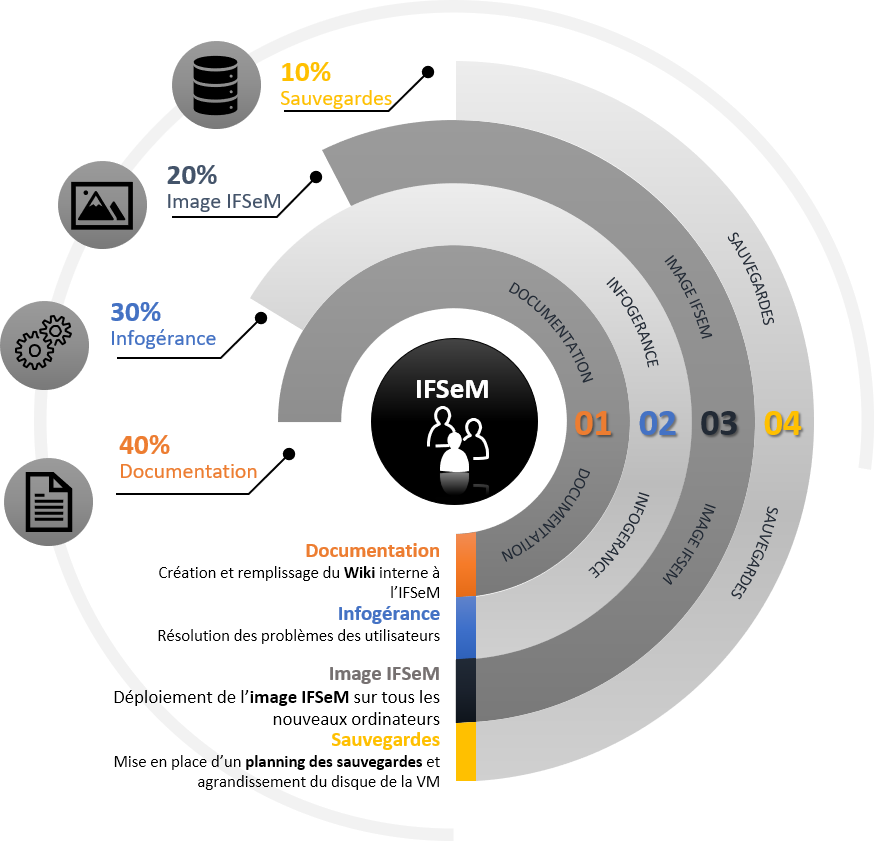
\includegraphics[width=15cm]{./images/temps.png}
}


\subsection{Hotline téléphonique et assistance aux utilisateurs }
Une importante partie du travail consistait en l'aide aux utilisateurs. De ce fait, en plus du système de ticketing évoqué précédemment, le pôle SI fait aussi office de centre hotline pour les utilisateurs. Tous les membres disposent d'un téléphone fonctionnant par téléphonie IP, permettant d'appeler n'importe quel agent du CNRS.

\subsubsection{L'infogérance}
Une fois que le problème est identifié (appel ou ticket), une phase de recherche commence. La première chose à vérifier est si ce problème a déjà été reporté et/ou si un problème proche a déjà été corrigé par le passé. Si c'est le cas, il faudra alors appliquer une GPO. Une GPO est une règle que l'on peut appliquer à différents niveaux. Tout cela demande une grande organisation. 
\medbreak
Un exemple concret que j'ai rencontré lors de mon stage est un problème qui survient lorsqu'une machine de la marque Hewlett-Packard Company (HP), se connecte à un VPN. Un processus en tâche de fond détecte la connexion VPN comme étant une connexion filaire et désactive automatiquement le Wifi, ayant pour effet de couper la connexion avec le VPN. La personne ne peut donc pas travailler de chez elle, car l'ensemble des applications nationales ne sont accessibles que depuis le réseau du CNRS, soit physiquement soit au travers d'un VPN. La solution consistait donc à arrêter ce processus dès le démarrage pour les machines HP.
\medbreak
En plus des GPO qui régissent le parc informatique, l'IFSeM dispose d'un serveur Dell, appelé K1000, permettant de gérer l'ensemble du parc informatique. Ce serveur permet de savoir exactement en temps réel qui est connecté sur quelle machine et à quelle heure. De plus, cela permet de gérer les mises à jour système et logiciel pour tout le monde. Le but étant qu'un utilisateur ne se rende compte de rien. Les mises à jour sont donc effectuées avec des options qui les rendent silencieuses, les grosses mises à jours étant effectuées de nuit\dots 

\subsubsection{Déploiement de l'image IFSeM}
En informatique, on parle  de deploiment d'image système ou d'image, un système d'exploitation (dans notre cas un système Windows 10 Pro) que l'on va déployer en grand nombre. On peut stocker une image sur un CD (comme les CD d'installation Windows), une clé USB ou encore sur un serveur depuis le réseau (cas du CNRS) à l'aide du protocole PXE. 
\medbreak
Lorsqu'une nouvelle machine (portable ou fixe) est livrée, il faut y installer dessus l'image standard créée par l'IFSeM. En effet, jusqu'à présent, chaque délégation possédait sa propre image, que le SSI local (service système d'information) déployait sur les machines qu'il recevait. Depuis quelques mois, il a été décidé de déployer une image unique sur tous les postes de chaque délégation francilienne, afin de faciliter le travail et la gestion à distance du parc informatique.
\medbreak
J'ai donc dû me déplacer, avec l'équipe Gestion des Infrastructures sur le site de la délégation de Meudon (en annexe l'ordre de mission validée par le service des stages), afin de déployer des images systèmes et installer les postes qui venaient d'être livrés. Cela permet de mieux gérer l'infrastructure de l'ensemble des postes. Cette intervention sur un autre site que celui de Villejuif m'a permis de découvrir un autre environnement de travail et de me rendre compte des contraintes opérationnelles, techniques et d’approvisionnement des interventions sur un autre site. En effet, en plus des problèmes réseaux, nous avons du attendre que le matériel demandé arrive car il n'avait pas été préparé en amont par le SSI local. 

\subsection{Maintien des applications nationales : MCO-Linux}
Une des activités que j'ai effectué durant ce stage était du MCO-Linux (Maintien en Conditions Opérationnelles). Cela consiste à assurer une continuité de service et une disponibilité des services hébergés sur les hyperviseurs. \\
La plupart des services sont hébergés sur des hyperviseurs, eux même divisés en plusieurs machines virtuelles. Il faut alors impérativement garantir une accessibilité à ces services. Lors d'un bug, nous devions basculer sur le serveur de secours, afin que les utilisateurs ne se rendent pas compte du problème, puis corriger ce dernier. Cette tâche dépendait complètement du type de service et du type de bug. Le plus souvent, un simple reboot de la VM (Virtual-Machine), l'observation des logs (journaux tenus à jour par la machine), ou même une restauration à une version antérieure suffisait à résoudre le problème. 

\subsection{Sauvegardes des machines virtuelles}
L'IFSeM disposait d'un serveur de stockage permettant de stocker les sauvegardes des différentes applications. Ce serveur (qui est en réalité une VM), fait tourner l'application BackUpPC, une application avec une interface web permettant de gérer les sauvegardes de toutes les VM. La place étant limitée, un système de roulement des sauvegardes est mis en place automatiquement par BackUpPC, afin de ne conserver que certaines sauvegardes (partielles et totales). \\
J'ai mis en place un planning des sauvegardes (pourquoi). Une autre tache que j'ai effectuer fût d'augmenter la place du serveur de sauvegarde. En effet, plus le temps passait, plus les sauvegardes était lourdes. Le serveur à finit pas être plein. On a donc sollicité mon aide afin d'augmenter la taille de la partition du disque virtuel accessible depuis la VM, sans pour autant écraser les sauvegardes. Après avoir, pendant une journée, reproduit la situation sur un environnement de test, j'ai réussi sans encombre l'agrandissement de la partition, qui est une opération qui peut s'avérer périlleuse, d'autant plus que seuls les outils en ligne de commande étaient disponibles : Parted, resize ...

\subsection{La documentation}
Une autre partie de mon travail durant ce stage fut de compléter la documentation. En effet, chacune des équipes du pôle SI possédait sa propre documentation, souvent au format Word ou même bloc-note. Un projet en cours lors de mon arrivée était de regrouper toute la documentation sur un Wiki accessible par tout le pôle SI de l'IFSeM. J'ai donc dû recopier et transférer les documents depuis les fichiers Word vers le Wiki. \\
De plus, afin de vérifier que les informations étaient correctes, il m'a été demandé de suivre et d'exécuter les tâches décrites dans les documentation pour les vérifier et de prendre des captures d'écran des messages affichés pour l'illustrer. 
Ce travail m'a occupé environ 40\% de mon temps. Bien que peu intéressante et très chronophage, cette tâche est pourtant nécessaire et permet aux employés de gagner beaucoup de temps par la suite.
